% Part: biographies 
% Chapter: georg-cantor 
% Section: biography
\documentclass[../../../include/open-logic-section]{subfiles}

\begin{document}

\olfileid{bio}{gec}{bio} 
\olsection{Biography}

\begin{figure}[h!] 
\centering 
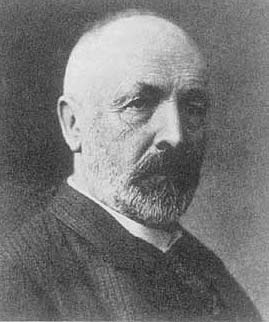
\includegraphics[scale=.75]{georg-cantor.png}
\caption{Georg Cantor. Photo Credit: Wikimedia Commons.} 
\end{figure}

Much falsity has been published about Georg Cantor's life. An early
biographical work, for instance, claimed that Georg was born and found on a
ship that was sailing for Saint Petersburg, Russia, and that his parents
were unknown \citep[352]{Grattan-Guinness1971}. This, of course, is not
true, although he was born in Saint Petersburg in 1845.

Cantor recieved his Ph.D. in mathematics at the University of Berlin in
1867. He is known for his work in set theory, and is credited with making
set theory an active research discipline \citep[353]{Grattan-Guinness1971}.
He was the first to prove that there are infinite sets of different sizes.
His theories, and especially his theory of infinities, caused much debate
among mathematicians, and his work was rarely accepted
\citep[353]{Grattan-Guinness1971}. For this reason, he never recieved a
position as a prestigious univeristy, and spent his entire career at the
Univeristy of Halle.

Cantor's personality is of interest to those interested in his mathematical
works. His religious beliefs and his mathematical work were inextricably
tied; he even claimed that the theory of transfinite numbers had been
communicated to him directly by God. \citep[8]{Dauben2004}. In later life,
Cantor suffered from mental illness. Beginning in 1984, and more frequently
towards his later years, Cantor was commited to a sanitorium due to
depression. The heavy criticism of his work, including a falling out with
mathematician Leopold Kronecker, led to his depression and a lack of
interest in mathematics. During times of depression, Cantor would turn to
philosophy and literature, even publishing a theory that Francis Bacon
actually penned Shakespeare's plays!

Cantor passed away quietly on January 6, 1918 in a sanitorium in Halle.

\begin{reading} 
\begin{itemize} 
\item For a full biography of Cantor, see
\citet{Dauben1990} and \citet{Grattan-Guinness1971}

\item For more information about Cantor's radical views, check out BBC
Radio 4's program \emph{A Brief History of Mathematics}. See
\citet{Sautoy2014}.

\item If you'd like to hear about Cantor's theories in rap form, see
\citet{Rose2012}.

\end{itemize} 
\end{reading}

\end{document}